\subsection{Data Analysis}

The data that is made available to develop a classifier is made up of a training set with 61878 items and a testing set with 144368 items. Each item has an ID, 93 features and a label (only in the training set). It is not known what the features represent, there are simply 93 of them and their value ranges depending on which feature it is. The minimum value for each one is 0 and the maximum value an be found in figure \ref{fig:max_per_feature}. As it can be seen, maximum values per feature are different for the training and testing set.
\begin{figure}[h!]
    % \centering
    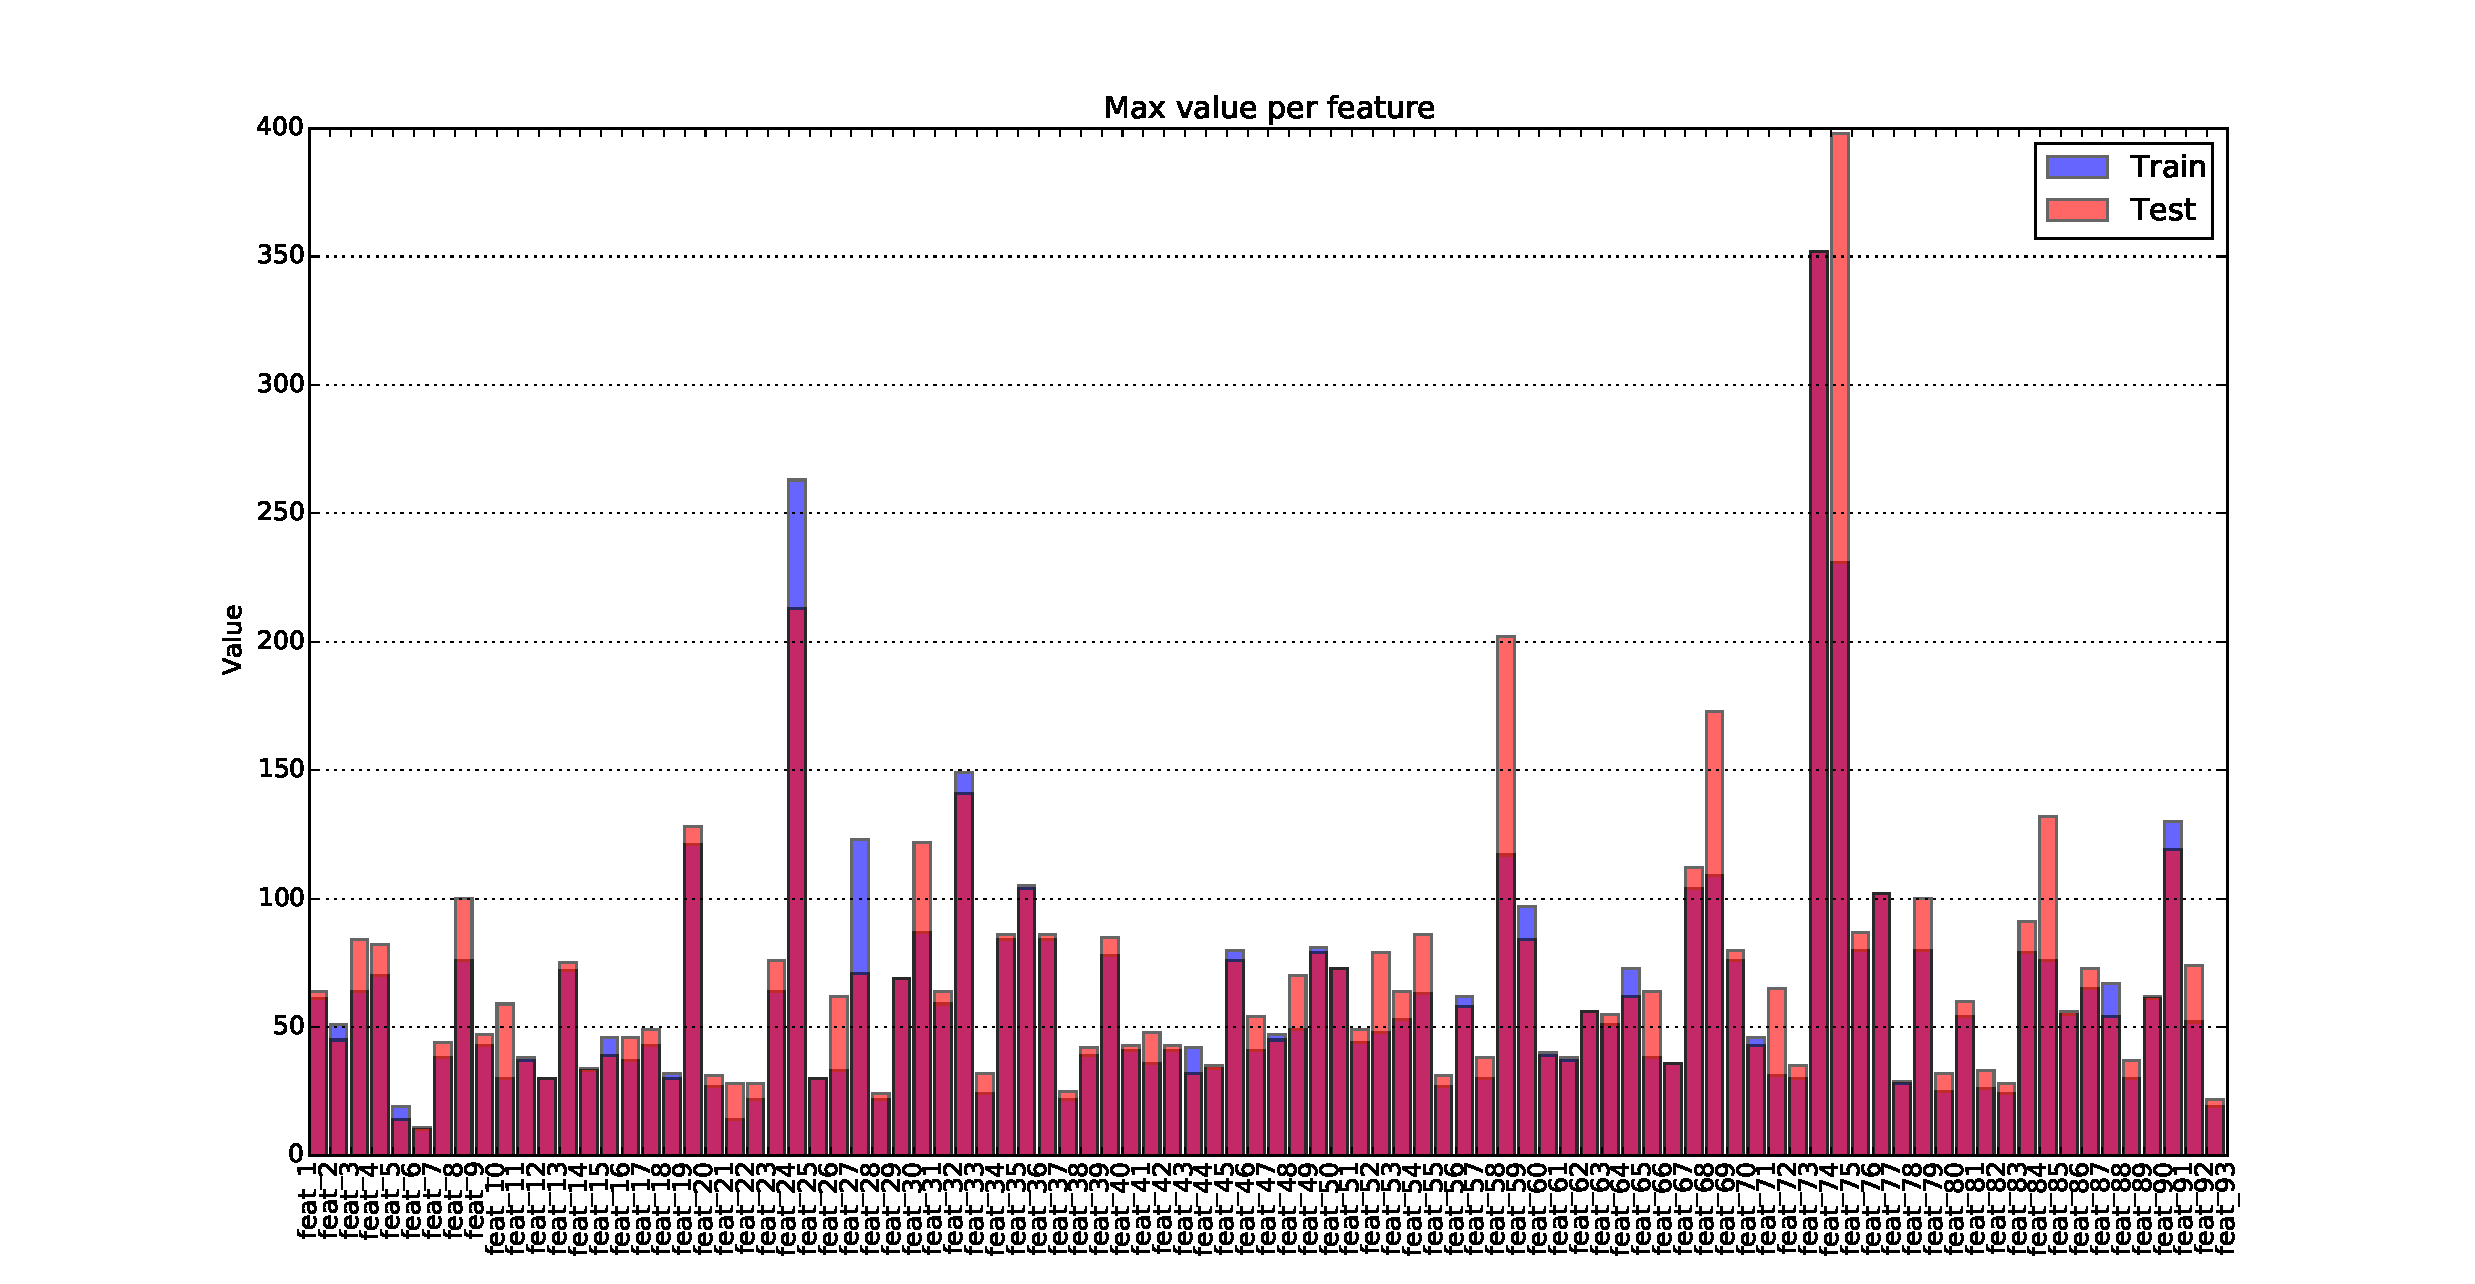
\includegraphics[trim={3.7cm 0cm 0.7cm 0.7cm},clip, width=1.1\textwidth]{max_per_feature}
    \caption{Maximum values per feature}
    \label{fig:max_per_feature}
\end{figure}

There are 9 different classes in which Otto wants its products classified. As with the features it is unknown what these classes represent.

As an attempt to visualize this high-dimensional data, the t-distributed stochastic neighbor embedding algorithm was used. It models each high-dimensional object by a two- or three-dimensional point in such a way that similar objects are modeled by nearby points and dissimilar objects are modeled by distant points.
\begin{figure}[h!]
    \centering
    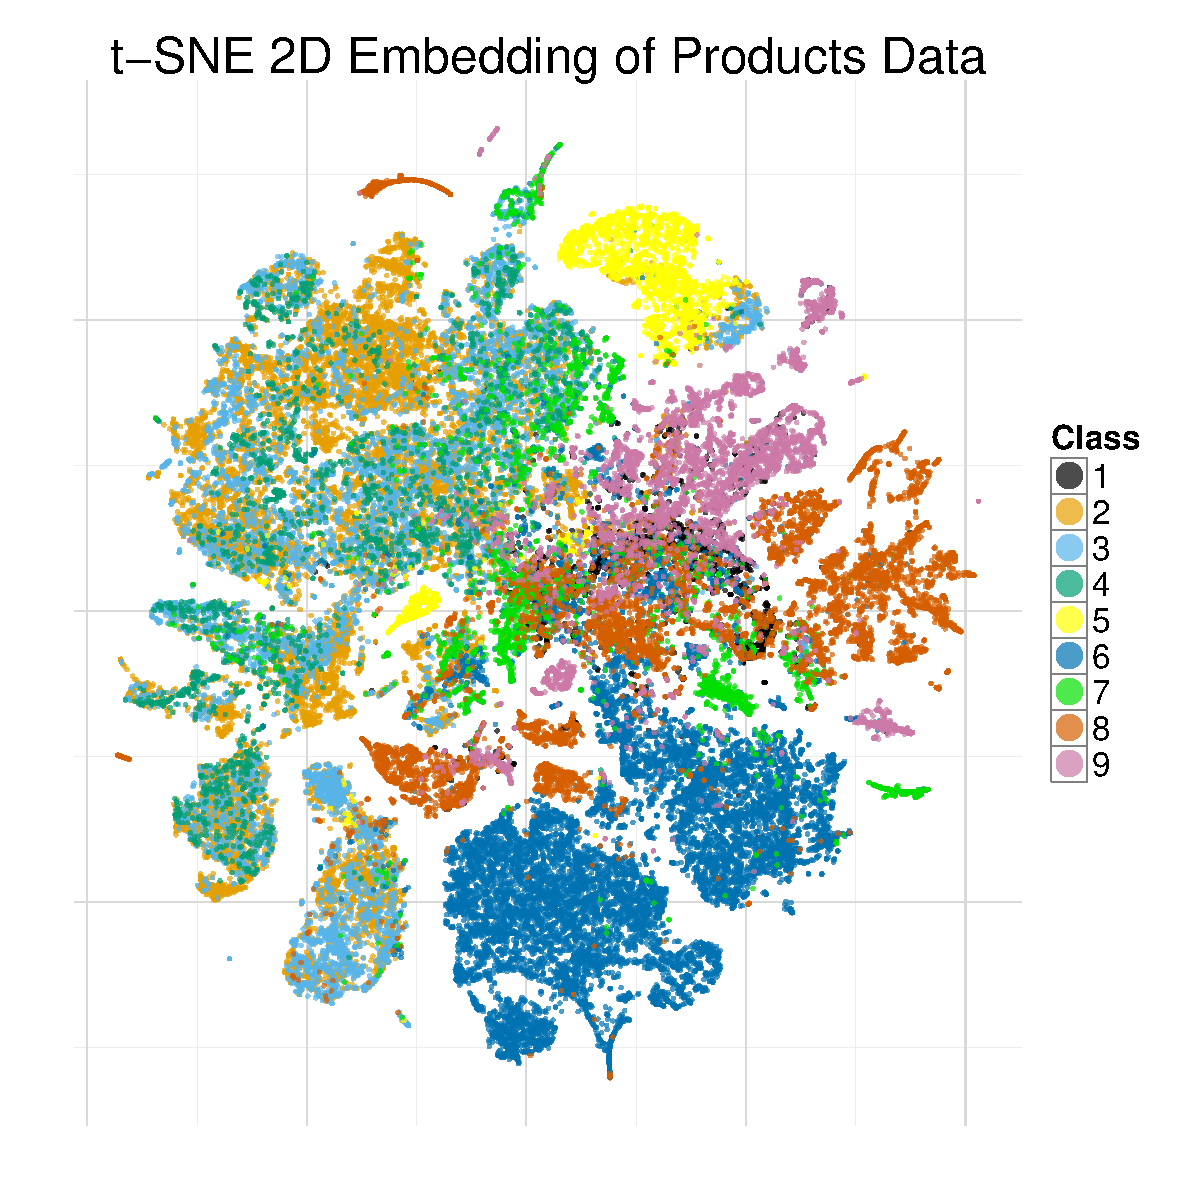
\includegraphics[width=0.9\textwidth]{tsne}
    \caption{t-distributed stochastic neighbor embedding}
    \label{fig:Tsne}
\end{figure}

From the result it can be seen that some samples will be most likely misclassified. Meaning that achieving a low logarithmic loss won't be easy.
\subsection{Research}
To find the most suitable machine learning algorithm for the classifying of Otto items we start by researching known algorithms. The most promising of the ones found are:
\begin{itemize}
\item Logistic regression
\item K-nearest neighbor
\item Random Forests
\item Gradient Boosting
\end{itemize}
All except Logistic Regression and K-nearest neighbor are ensemble methods, meaning that they are combinations of multiple machine learning algorithms. Ensemble methods often have better performance because they are more flexible due to the fact that they are combinations of several algorithms.\\
\subsubsection{Logistic Regression}
Logistic Regression is a direct probability model that was developed by statistician D. R. Cox in 1958. The probabilities describing the possible outcomes of a single trial are modeled, as a function of the predictor variables, using a logistic function. 

Logistic regression can be seen as a special case of generalized linear model and thus analogous to linear regression. However, The model of logistic regression is based on quite different assumptions, First, the conditional distribution $p(y|x)$ is a Bernoulli distribution rather than a Gaussian one, because the dependent variable is binary. Second, the estimated probabilities are restricted to $[0,1]$ through the logistic distribution function because it predicts the probability of the instance being positive.
\begin{figure}[h!]
	\centering
	\includegraphics[width=0.7\textwidth]{logistic_curve}
	\caption{Logistic function $\sigma(t)$}
	\label{fig:log_curve}
\end{figure}

Multinomial logistic regression is used when having multiple classes. This involves all classes uniformly by using the $softmax$ function (Bridle 1990). This boosts the weighted sum for one class through exponentiation and normalization so that it's corresponding output value is close to $1$.
\subsubsection{K-nearest neighbor}
 the k-Nearest Neighbors algorithm (k-NN) is a non-parametric method used for classification and regression. The input consists of the k closest training examples in the feature space and for k-NN classification the output is a class membership. A sample is assigned to the class most common among its $k$ nearest neighbors. k-NN is a type of lazy learning, where the function is only approximated locally and all computation is deferred until classification. It is one of the simplest of all machine learning algorithms. 
 
 It can be useful to assign weight to the contributions of the neighbors, so that the nearer neighbors contribute more than others. This can be achieved by using distant metrics (euclidean, manhattan, chebyshev).
\subsubsection{Random Forests}
Random Forests are similar to Bagging in the way that they have a similar basis. Both generate a number of trees of which each is constructed with a different sample of data and that give extra weight to points that were incorrectly classified. In Bagging the trees are independent from each other meaning newer trees are not dependent on earlier trees, they are constructed independently.

In Random Forests there is an extra layer of randomness in the method of constructing the classification trees. Instead of splitting each node and choosing the best from among all of the predictors, Random Forests split each node based on a randomly chosen subset of predictors. This might seem counter-intuitive but it actually appears to be robust against overfitting and it performs well.
\subsubsection{Gradient Boosting}
Gradient boosting is a machine learning technique for regression and classification problems, which produces a prediction model in the form of an ensemble of weak prediction models, typically decision trees.

Like other boosting methods, gradient boosting combines weak learners into a single strong learner, in an iterative fashion.
At each stage $1 \le m \le M$ of gradient boosting, it may be assumed that there is some imperfect model $F_m$. The gradient boosting algorithm does not change $F_m$ in any way; instead, it improves on it by constructing a new model that adds an estimator $h$ to provide a better model $F_{m+1}(x) = F_m(x) + h(x)$. In order to find $h$ we assume that a perfect solution would imply

    $$ F_{m+1} = F_m(x) + h(x) = y $$

or, equivalently,

    $$ h(x) = y - F_m(x) $$

Therefore, gradient boosting will fit $h$ to the residual $y - F_m(x)$. Like in other boosting variants, each $F_{m+1}$ learns to correct its predecessor $F_m$. Gradient boosting is a gradient descent algorithm; and generalizing it involves "plugging in" a loss function and its gradient.